\documentclass[tikz]{standalone}
\usepackage{mathpazo}
\usepackage{siunitx}
\usepackage{sankey}
\usepackage[european resistors]{circuitikz}

\begin{document}

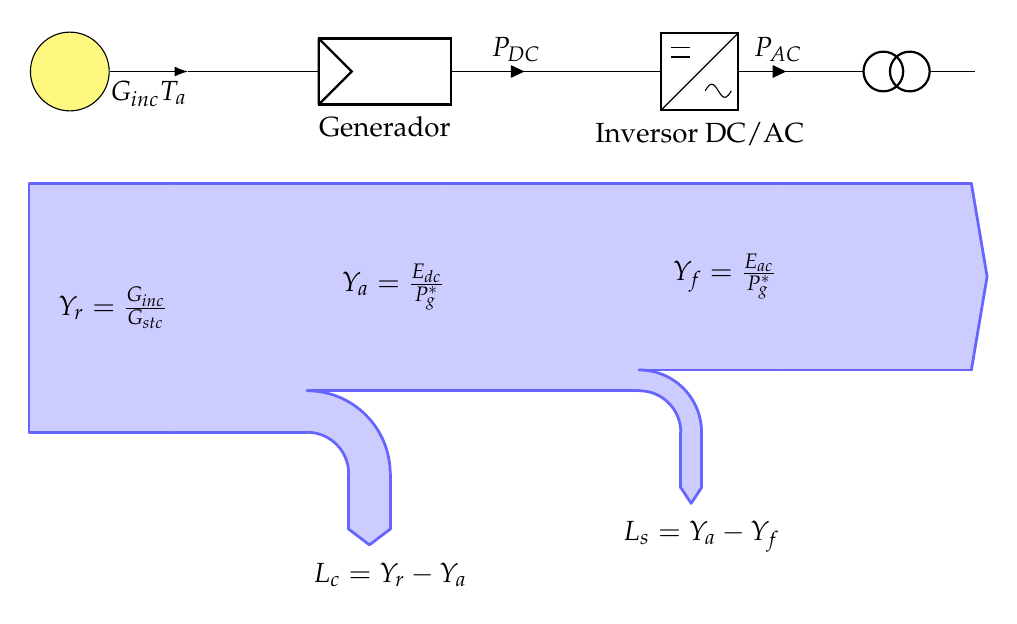
\begin{tikzpicture}
  \begin{scope}[shift={(0,3)}]
    \draw (0.5,0) node[draw, fill=yellow!50!white, circle, minimum size=1cm] (Sun) {};
    \draw[-Latex] (Sun) -- node[below] {$G_{inc} T_a$} ++(1.5,0) coordinate (A);
    \draw (A) to [pvmodule, invert, l_= Generador, i^>= $P_{DC}$] (7,0)
    to[sdcac, l_ = Inversor DC/AC, i = $P_{AC}$] (10,0)
    (10,0) to [oosourcetrans, n = T] (12,0);
  \end{scope}
\begin{sankeydiagram}
      \colorlet{cold}[rgb]{blue!20!white}
      \sankeyset{
        ratio=90pt/6,
        minimum radius=15pt,
        start style=simple,
        end style=simple,
        draw/.style={ draw=blue!60!white, line
          width=1pt,line cap=round,line join=round, },
        cold/.style={
          fill/.style={ draw=cold,line width=0pt,fill=cold, }, },
      }
      \sankeyset{cold}
      \sankeynodestart{name=Yr,at={0,0},angle=0,quantity=6}
      \sankeyadvance{Yr}{50pt}
      \node[anchor=east,align=center,inner xsep=0] at (Yr) {$Y_r = \frac{G_{inc}}{G_{stc}}$};
      \sankeyadvance{Yr}{50pt}
      \sankeyfork{Yr}{5/Ya,1/Lc}
      \sankeyadvance{Ya}{50pt}
      \node[anchor=east,align=center,inner xsep=0] at (Ya) {$Y_a = \frac{E_{dc}}{P^*_g}$};
      \sankeyadvance{Ya}{70pt}
      \sankeyturnright{Lc}{90}
      \sankeyadvance{Lc}{20pt}
      \sankeyend{Lc}
      \node[below, yshift = -3mm] at (Lc.north) {$L_c = Y_r - Y_a$};
      \sankeyfork{Ya}{4.5/Yf,0.5/Ls}
      \sankeyadvance{Yf}{50pt}
      \node[anchor=east,align=center,inner xsep=0] at (Yf) {$Y_f = \frac{E_{ac}}{P^*_g}$};
      \sankeyadvance{Yf}{70pt}
      \sankeyend{Yf}
      \sankeyturnright{Ls}{90}
      \sankeyadvance{Ls}{20pt}
      \sankeyend{Ls}
      \node[below, yshift = -3mm] at (Ls.north) {$L_s = Y_a - Y_f$};
    \end{sankeydiagram}

\end{tikzpicture}
\end{document}